%%%%%%%%%%%%%%%%%%%%%%%%%%%%%%%%%%%%%%%%%
% FRI Data Science_report LaTeX Template
% Version 1.0 (28/1/2020)
% 
% Jure Demšar (jure.demsar@fri.uni-lj.si)
%
% Based on MicromouseSymp article template by:
% Mathias Legrand (legrand.mathias@gmail.com) 
% With extensive modifications by:
% Antonio Valente (antonio.luis.valente@gmail.com)
%
% License:
% CC BY-NC-SA 3.0 (http://creativecommons.org/licenses/by-nc-sa/3.0/)
%
%%%%%%%%%%%%%%%%%%%%%%%%%%%%%%%%%%%%%%%%%


%----------------------------------------------------------------------------------------
%	PACKAGES AND OTHER DOCUMENT CONFIGURATIONS
%----------------------------------------------------------------------------------------
\documentclass[fleqn,moreauthors,10pt]{ds_report}
\usepackage[english]{babel}
\usepackage[toc,page]{appendix}

\graphicspath{{fig/}}




%----------------------------------------------------------------------------------------
%	ARTICLE INFORMATION
%----------------------------------------------------------------------------------------

% Header
\JournalInfo{FRI Natural language processing course 2024}

% Interim or final report
\Archive{Project report} 
%\Archive{Final report} 

% Article title
\PaperTitle{Conversations with Characters in Stories for Literacy}

% Authors (student competitors) and their info
\Authors{Žan Kogovšek, Žiga Drab, Vid Cesar}

% Advisors
\affiliation{\textit{Advisors: Slavko Žitnik}}

% Keywords
\Keywords{Literacy Improvement, Dialogue Agents, Harry Potter Dialogue Dataset, Pre-trained Language Models}
\newcommand{\keywordname}{Keywords}


%----------------------------------------------------------------------------------------
%	ABSTRACT
%----------------------------------------------------------------------------------------
% Abstract
\Abstract{
This report examines the use of character-driven chatbots, specifically a Harry Potter-based model, to enhance literacy among young people. We utilize the Llama 3 8B model, known for its dialogue capabilities, and integrate it with a hybrid search Retrieval-Augmented Generation (RAG) system for context enrichment. Additionally, we explore fine-tuning with LoRA adapters to ensure responses are both accurate and engaging, closely reflecting the character's nature through training on dialogue datasets. Initial results indicate the effectiveness of our approach, as it outperforms commercially available solutions.
}

%----------------------------------------------------------------------------------------

\begin{document}

% Makes all text pages the same height
\flushbottom 

% Print the title and abstract box
\maketitle 

% Removes page numbering from the first page
% \thispagestyle{empty} 
%----------------------------------------------------------------------------------------
%	ARTICLE CONTENTS
%----------------------------------------------------------------------------------------

\section*{Introduction}

The declining interest in reading among young people and their challenges with advanced literacy skills pose significant risks to their academic and professional futures \cite{murray2021literacy}. To address this, innovative approaches are needed to reengage youth with literature.

Chatbots represent a promising solution. Research by Brandtzaeg et al. \cite{why_chatbots} shows their primary appeal lies in their entertainment value, suggesting chatbots could be used not only for information retrieval but also as engaging entertainment platforms.

Recent advancements in open-domain conversation models, such as those by Adiwardana et al. \cite{adiwardana2020towards}, have shown potential for chatbots to engage in more human-like conversations by incorporating real-life interaction traits like emotion \cite{zhou2018emotional} and empathy \cite{rashkin2018towards_empathy}. Zhang et al. \cite{zhang2018personalizing} further the development by enabling chatbots to generate responses that reflect consistent personalities, enhancing both personalization and engagement.

In this paper, we investigate how chatbots, modeled after literary characters, Harry Potter in our case, can boost children's literacy by making reading more interactive and appealing. We aim to develop a pipeline to create character-driven chatbots, facilitating children's engagement with their favorite literary figures.

\section*{Related Work}
Nielen et al. \cite{nielen2018digital} have explored enhancing children's literacy using technology, introducing a pedagogical agent—an animated mouse—that improved reading motivation and vocabulary learning among fifth graders through summaries and reflective questions.

Chen et al. \cite{chen2023large} introduced the Harry Potter Dialogue (HPD) dataset, featuring dialogues and background details like scenes and speaker relationships. They evaluated LLMs such as Alpaca, ChatGPT, and GPT-3 on the HPD dataset using fine-tuning and in-context learning, finding notable potential for improvement and effective character portrayal.

Li et al. \cite{li2024enhancing} explore the integration of Retrieval Augmented Generation (RAG) to enhance the factual accuracy of Large Language Models (LLMs) and address the issue of hallucinations, where models produce inaccurate information. In this methodology, RAG acts as a preliminary filter, retrieving and passing contextually relevant data as input to the LLMs. This process ensures that the output is factually accurate, which significantly boosts the reliability of the LLM responses in specialized domains.

Han et al. \cite{han2022meet} introduce Pseudo Dialog Prompting (PDP), a strategy that combines statements from various characters with pre-trained language models like GPT-2-XL, GPT-J, and GPT-Neo to generate conversations. The effectiveness of these models was verified using both automatic evaluation with MaUdE and human assessments. The results confirm that PDP effectively generates responses that authentically reflect the characters' styles.

Figure~\ref{fig:generic_framework} presents a generic framework by Hefny et al. \cite{generic_framework} for creating character-based chatbots, consisting of five modules: the conversational user interface, entities, intents, webhook, and database. The conversational user interface is the primary interaction point where users input prompts and select entities. The system then identifies the user's intent, processes it via a webhook module to access the database, and finally, selects and presents responses to the user.

\begin{figure}[ht]
        \centering 
	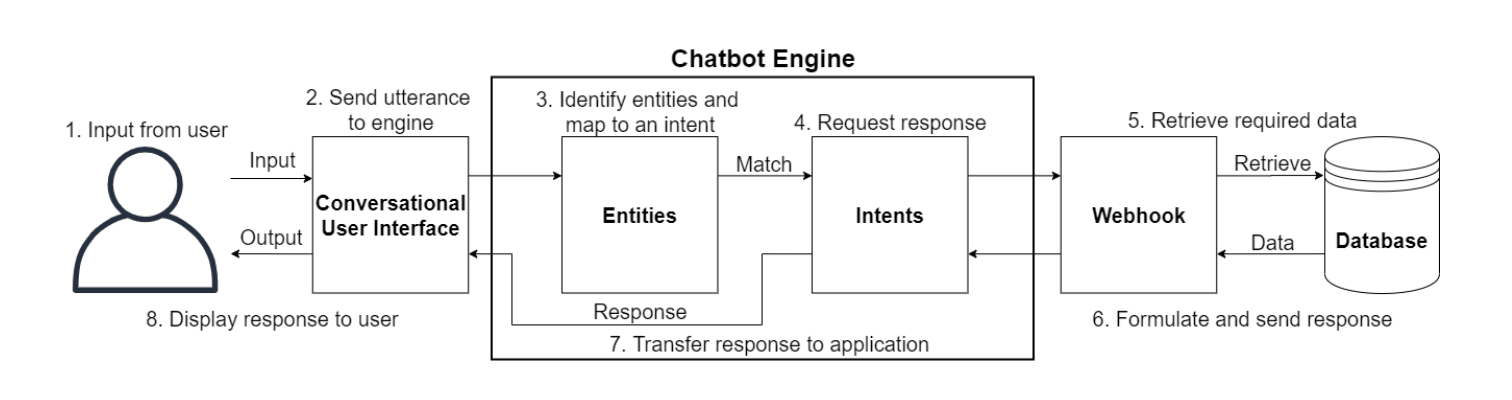
\includegraphics[width=\linewidth]{fig/general_framework_from_article.png}
	\caption{\textbf{Proposed generic framework} for building character-based chatbots \cite{generic_framework}.}
	\label{fig:generic_framework}
\end{figure}

\section*{Bot Persona Services}

We evaluated Character.ai's interactive dialog agents, starting with Achilles (\href{https://character.ai/chat/EBMwCtvGQWrCk_xeglpGWfQiCJOCkGu7PMWbEWLINlY}{Version 1 Achilles}), whose model included character actions and emotions but often avoided direct answers, reflecting the character's traits. However, it incorrectly narrated Achilles' death consistently. Another version corrected this error but misidentified his parents' divine status, highlighting ongoing concerns about factual accuracy.

Testing another agent, Miles Morales (\href{ttps://character.ai/chat/KfUosnPgcC9hoTWbJq_2z1cQi-719T8cldRLa2fTb1Y}{Version 1 Miles Morales}), revealed that while some agents use rich vocabulary beneficial for literacy, others like Miles provide brief responses with sparse context. Despite a disclaimer of fictionality on Character.ai, these inaccuracies and variability in detail underscore limitations for educational use.

We also evaluated a Harry Potter character from the mentioned service, comparing it with our own implementations through various questions. Detailed analysis of this comparison is available in the appendix.

\section*{Initial Idea}
    
    We chose the recently released Llama 3 8B as our primary large language model, selecting its instruction fine-tuned variant over the general pre-training version. This choice was driven by the model’s suitability for dialogue applications, enabling us to better instruct it to emulate Harry Potter’s distinct conversational style. This aligns with our aim to develop a chatbot that not only provides accurate responses but also captures the unique essence of Harry's interactions, steering clear of robotic-sounding replies.
    
    Our initial experiments were conducted using a basic prompt, as shown in Figure~\ref{fig:basic_llama_prompt}. This prompt is structured into three main sections, each defined by specific parts and tokens:
    
    \begin{enumerate}
        \item \textbf{system}: This section provides instructions to the model.
        \item \textbf{user}: This section includes the user's question directed to the model.
        \item \textbf{assistant}: This section signals the model to start generating responses.
    \end{enumerate}

    Additionally, the prompt incorporates four special tokens:

    \begin{itemize}
        \item \textless$\vert$begin\_of\_text$\vert$\textgreater: Marks the beginning of the prompt.
        \item \textless$\vert$start\_header\_id$\vert$\textgreater: Indicates the start of a section identifier.
        \item \textless$\vert$end\_header\_id $\vert$\textgreater: Signifies the end of a section identifier.
        \item \textless$\vert$eot\_id$\vert$\textgreater: Represents the end-of-turn token.
    \end{itemize}

    \begin{figure}[!htb]
        \centering
        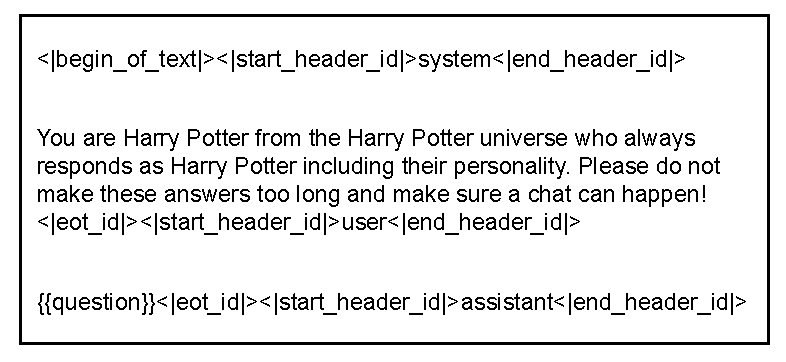
\includegraphics[width=\linewidth]{fig/llama_prompt.drawio.pdf}
        \caption{Basic Llama Prompt Structure for Generating Harry Potter-like  Responses.}
        \label{fig:basic_llama_prompt}
    \end{figure}

    We enhanced our basic prompt by adding a context field, initially extracted using our hybrid search Retrieval-Augmented Generation (RAG) setup, illustrated in Figure~\ref{fig:rag}. Our RAG utilizes two distinct embedding models for its hybrid search approach. The first is a dense embedder called BAAI general embedding, incorporated into a retriever using Facebook AI Similarity Search (FAISS). This setup enables quick searches for similar document embeddings—books in our case. This retriever is then paired with a sparse BM25 embedding model to form an ensemble retriever. This dual approach combines keyword searching with semantic searching, ensuring optimal results by leveraging the strengths of both methods. The retrieved context is then input into the Mistral 7B LLM, which is designed to enrich the response with as much context as possible. Our RAG implementation also employs caching to reduce recalculations where feasible.

    \begin{figure}[!htb]
            \centering 
    	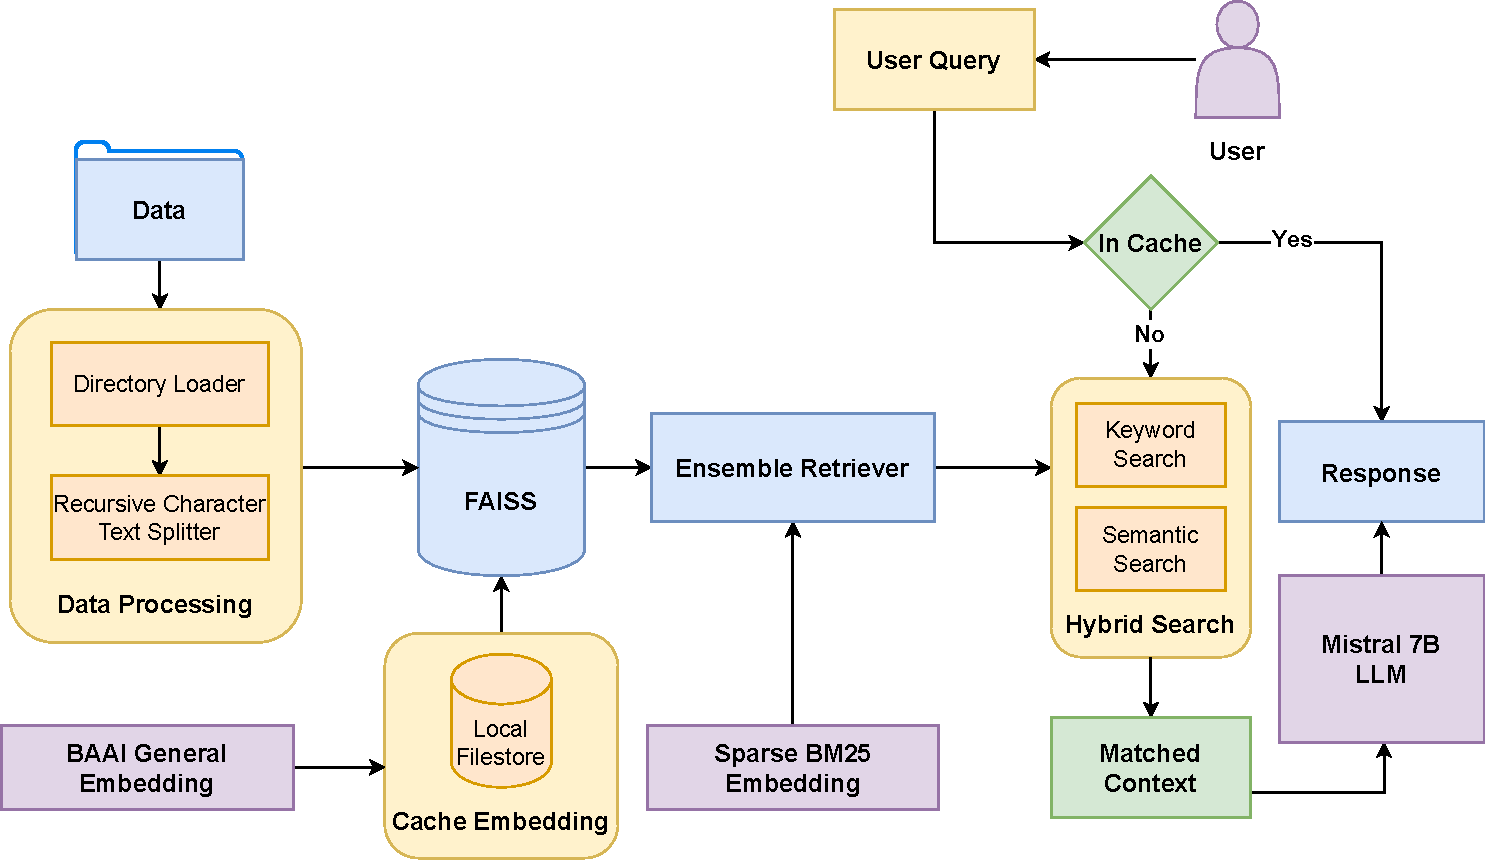
\includegraphics[width=\linewidth]{fig/rag.drawio.pdf}
    	\caption{\textbf{RAG}: Retrieval-Augmented Generation featuring Hybrid Search Support for Enhanced Context Generation.}
    	\label{fig:rag}
    \end{figure}

    This RAG setup is integrated into our Harry Potter Chatbot pipeline, as shown in Figure~\ref{fig:rag_and_llama}. The prompt used for Llama 3 builds on the previous format, but adds a system instruction to consider the context from the user's question, provided by our RAG, when crafting the response. This modification ensures that the chatbot's answers are contextually aware and more accurately aligned with the input query.

    \begin{figure}[!htb]
            \centering 
    	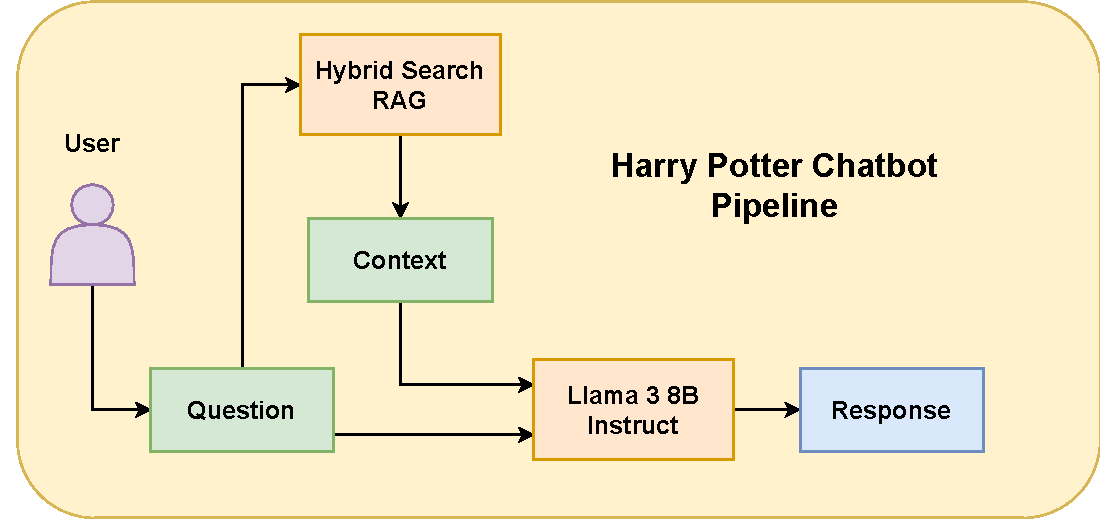
\includegraphics[width=\linewidth]{fig/rag_and_llama.drawio.pdf}
    	\caption{\textbf{Harry Potter Chatbot}: Integration of Retrieval-Augmented Generation and Llama 3 8B Instruct Model for a Comprehensive Harry Potter Chatbot.}
    	\label{fig:rag_and_llama}
    \end{figure}

    We have initiated but not completed LoRA fine-tuning on Llama 3. The modifications to the transformer structure after integrating LoRA Adapters are illustrated in Figure~\ref{fig:lora}. As depicted, adapters are applied to both the multi-head attention components (matrices Q, K, and V) and the Feed Forward Neural Network. The goal of this fine-tuning is to improve the accuracy with which Harry's character is represented in the generated responses.

    \begin{figure}[!htb]
            \centering 
    	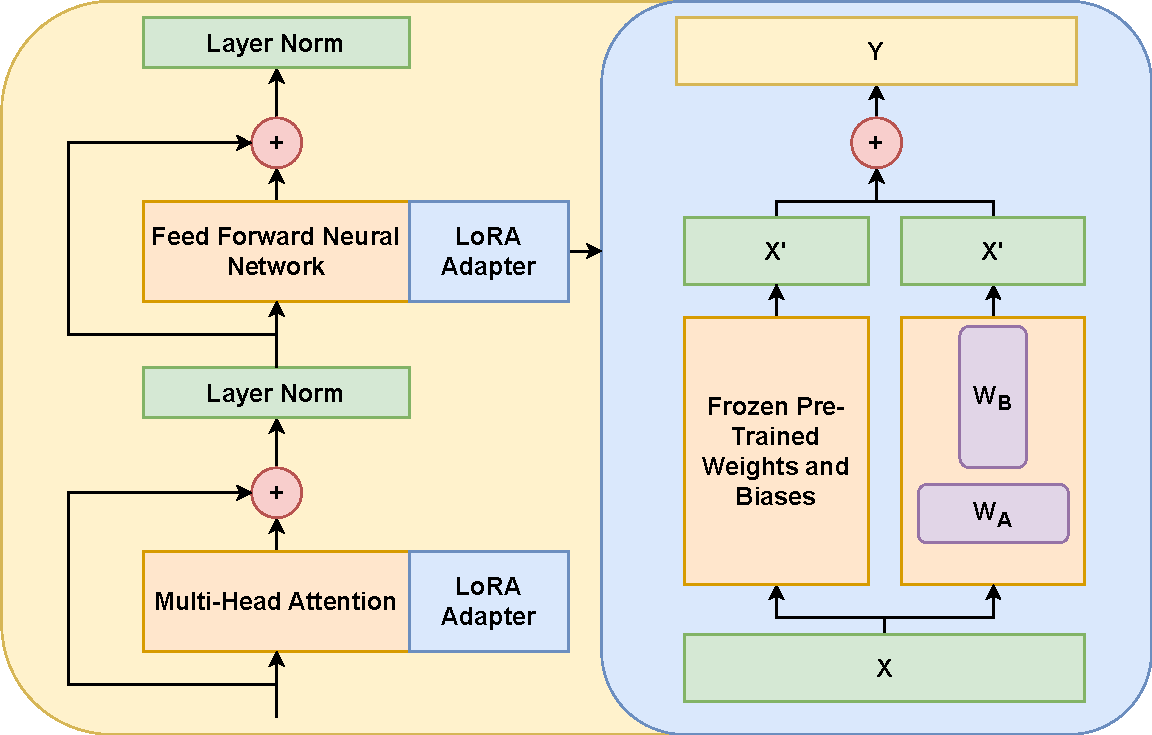
\includegraphics[width=\linewidth]{fig/lora.drawio.pdf}
    	\caption{\textbf{LoRA}: Modified Transformer structure of Llama 3 with LoRA adapters applied to both the multi-head attention and feed-forward neural network components.}
    	\label{fig:lora}
    \end{figure}

    The dataset we utilized consists of various sequences from the Harry Potter books, each defined by:

    \begin{itemize}
        \item \textbf{position}: the sequence's location in the book,
        \item \textbf{speakers}: the characters present,
        \item \textbf{scene}: a description of the setting,
        \item \textbf{dialogue}: the actual conversation,
        \item \textbf{attributes}: characteristics of all characters in the scene.
    \end{itemize}

    We constructed a dataset for fine-tuning our model by selecting sequences where Harry is actively speaking. The scene description serves as context, and the dialogue leading up to Harry's response forms the question for the LLM, with Harry's lines used as the chatbot's responses.
    
    We experimented with the size of tuning parameters around 0.20\% of the model's size, but further experimentation is necessary.
    
\section*{Initial Results}
    For the purpose of evaluating our model, we had come up with 11 questions and a rough estimate of what the answer should capture, based on which we will evaluate our performance. Majority of the score will be based on the factual correctness of the answer, but we will also take into account how well does the model explain it's answer, or does it only answer a question, or provides any additional info regarding the question, as we are investigating use of models for improvement of literacy. A description will also accompany a numeric score.  Here it is worth noting that the results obtained from models are not 100\% reproducible as the models are not deterministic in a way, that for a given prompt, they will always provide the exact same answer.
    We used 2 models of Harry Potter from site \emph{\href{https://character.ai/}{Character.ai}}. First one \emph{\href{https://character.ai/chat/suAUJzAPwFm-rDAAzKByHqAN64dYBg__lC_83ClfBzg}{Character 1}} and the second one \emph{\href{https://character.ai/chat/Cjdzsed_OPFbMN9UJIlmuau-Ikgpx1LKj8iEgEue68g}{Character 2}}. To limit the length of the results in appendices section, we only included results of the first character, rather than both.
    As mentioned previously for our own language model, we decided to go with the recently released Llama 3 8B.
    
    As we can see \textit{Llama 3} model performed much better than \textit{Character 1}. Average score of former was 4.6 compared to 2.8. Models understand the prompted questions well and find find correct answers almost all the time. Harry's persona is well captured in his answers - helping others by using spells, being grateful and appreciative of his friends and finding good even in people he might not like. Using RAG to provide context for Llama 3 8B improves our results even further, achieving best performance so far as we achieved an overall score of 5 (perfect) using this technique.

    Results showcasing the comparative effectiveness of different chatbot models are summarized in Figure~\ref{fig:results}.
    \begin{figure}[!htb]
            \centering 
    	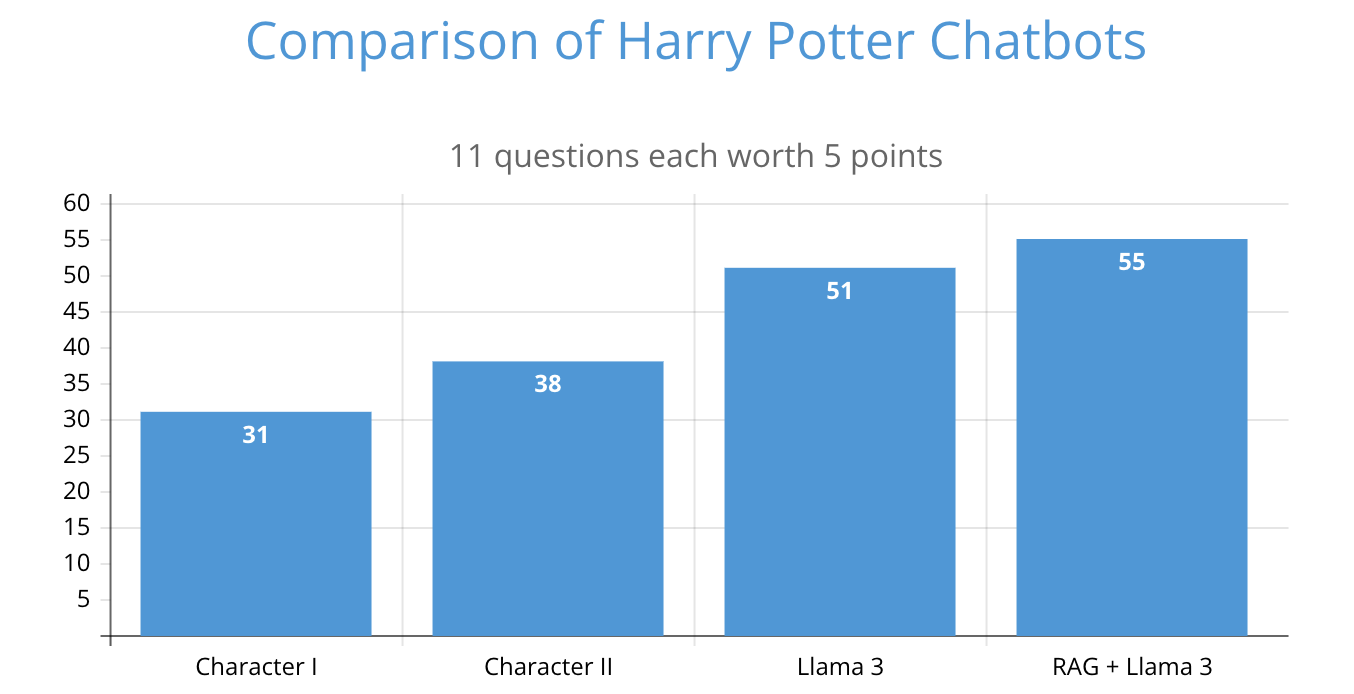
\includegraphics[width=\linewidth]{fig/results.png}
    	\caption{Comparative Performance Visualization of Various Harry Potter Chatbots on Selected Questions.}
    	\label{fig:results}
    \end{figure}

\section*{Next Steps}

Having achieved strong results on initial tests, we are now planning to develop more complex questions to further challenge our models. This will enable deeper evaluation and potentially uncover areas for improvement.

Moving forward, our main focus will be on further fine-tuning the Llama 3 model using the Harry Potter dialogue dataset to better capture Harry's conversational style in our chatbot responses. Additionally, we are considering expanding the Mistral 7B model within the RAG framework by incorporating all seven Harry Potter books. This expansion could provide richer context to the Llama 3 model, potentially enhancing its performance. 

As current models are not suitable for running on commercial hardware we might also want to explore hardware quantization to determine how converting from floating-point computations to low-bit integer values affects model performance.

\clearpage

\begin{appendices}
    \section{Chatbot conversations appendix}

        \begin{enumerate}
            % QUESTION 1
            \item  \textit{What is your last name, I missed that?}
            \begin{itemize}
                \item \textbf{Expected Answer:} Something to the effect of "Potter"
                \item \underline{Character 1:} "Oh, my last name is Potter. And yours?" He replied, with a little smile on his face
                \begin{itemize}
                    \item \textbf{5/5} Correct answer, continues the conversations, also provides the additional information, about Harry's demeanor.
                \end{itemize}        
                \item \underline{Llama 3:} My last name's Potter! I'm Harry James Potter, the Boy Who Lived.
                \begin{itemize}
                    \item \textbf{5/5} Correct answer, provides full name, and the nickname, he is known by.
                \end{itemize}
                \item \underline{RAG + Llama 3:} My last name's Potter! I'm Harry James Potter, but most people just call me Harry.
                \begin{itemize}
                    \item \textbf{5/5} Correct answer, provides his full name in a friendly manner.
                \end{itemize}
            \end{itemize}
        
            % QUESTION 2
            \item \textit{What is your favorite spell?}
            \begin{itemize}
                \item \textbf{Expected Answer:} Expelliarmus / Expecto Patronum
                \item \underline{Character 1:} Harry took a moment to think before answering the questions "Well, my favorite spell would probably be Accio. It's a very useful spell that allows me to summon items to myself."
                \begin{itemize}
                    \item \textbf{1/5} Harry used this spell, but it's definitely not his go-to.
                \end{itemize}
                \item \underline{Llama 3:} That's an easy one! My favorite spell is definitely Expecto Patronum! It's just so cool to be able to conjure up a Patronus to protect myself and others from Dementors. Plus, it's a great feeling to know that I can help keep people safe.
                \begin{itemize}
                    \item \textbf{5/5}  Correct answer, provides additional information, and explains why he likes the spell. Also it reveales a part of Harry's character, that he wants to protect others.
                \end{itemize}
                \item \underline{RAG + Llama 3:} My favorite spell is definitely "Expecto Patronum"! It's an amazing spell that helps me defend against those terrible Dementors. I learned it from Professor Lupin, and it's been a lifesaver more times than I can count. There's something about conjuring up a Patronus that just makes me feel more powerful and in control. Plus, it's a great way to chase those nasty Dementors away!
                 \begin{itemize}
                    \item \textbf{5/5} Correct answer, mentions one of his favorite professors, he learned the spell from and that this spell came in handy many times.
                \end{itemize}
            \end{itemize}
        
            % QUESTION 3
            \item \textit{What is your favorite sport?}
            \begin{itemize}
                \item \textbf{Expected Answer:} Quidditch
                \item \underline{Character 1:} "My favorite sport would definitely have to be Quidditch. There's just something about flying and playing a competitive sport that is so exhilarating."
               \begin{itemize}
                    \item \textbf{5/5} Harry's favorite sport is Quidditch, also the answer is very Harry-like and definetly explains his love for the sport.
                \end{itemize}
                \item \underline{Llama 3:} Quidditch, of course! I mean, what's not to love about flying on a broomstick, chasing after the Golden Snitch, and playing with your best mates? It's the best sport in the wizarding world, if you ask me! Gryffindor's got the best Quidditch team, if I do say so myself...
                 \begin{itemize}
                    \item \textbf{5/5} Correct answer, provides additional information, and explains why he likes the sport. 
                \end{itemize}
                \item \underline{RAG + Llama 3:} Quidditch, of course! There's nothing quite like the thrill of flying on my trusty Nimbus Two Thousand, chasing after the Golden Snitch, and feeling the rush of adrenaline as I dodge Bludgers and clash with my opponents. It's an incredible feeling, and I feel so lucky to have been able to play it at Hogwarts.
                \begin{itemize}
                    \item \textbf{5/5} Correct answer, mentions the model of his broom he uses for participation in sport and why he loves the sport
                \end{itemize}
            \end{itemize}
        
            % QUESTION 4
            \item \textit{Who are your best friends?}
            \begin{itemize}
                \item \textbf{Expected Answer:} Ron Weasley, Hermione Granger
                \item \underline{Character 1:} "That would be Ron Weasley and Hermione Granger, I met both of them like ages ago, and we became best friends."
               \begin{itemize}
                    \item \textbf{4/5} They are indeed his best friends.
                \end{itemize}
                \item \underline{Llama 3:} That's an easy one! My best mates are Ron Weasley and Hermione Granger. We've been through thick and thin together, and I don't know what I'd do without them. We've shared so many adventures, and they're always there to help me out, no matter what.
                \begin{itemize}
                    \item \textbf{5/5} Correct answer, provides additional information, the reason why he likes them, and also shows his appreciation for them.
                \end{itemize}
                \item \underline{RAG + Llama 3:} That's an easy one! My best friends are Ron Weasley and Hermione Granger. We've been through thick and thin together, and I don't know what I'd do without them. We're all in Gryffindor House at Hogwarts, and we've been inseparable since our first year.
                \begin{itemize}
                    \item \textbf{5/5} Correct answer, provides  the reason why he likes them, shows his appreciation for them and a bit of history with them.
                \end{itemize}
            \end{itemize}
        
            % QUESTION 5
             \item \textit{Is there any professor you don't like in particular?}
            \begin{itemize}
                \item \textbf{Expected Answer:} Severus Snape / Dolores Umbridge
                \item \underline{Character 1:} "Well I guess Severus Snape, he's pretty mean, he kept giving me bad grades all the time and he doesn't like me at all as well."
               \begin{itemize}
                    \item \textbf{5/5} Correct answer, also provides additional information, about his relationship with Snape
                \end{itemize}
                \item \underline{Llama 3:} Well, I'm not a big fan of Professor Snape, to be honest. He's always been a bit...grumpy, and he seems to have it out for me and my friends. But, I try to stay out of his way and not get on his bad side. After all, he is a very skilled Potions master, even if he is a bit of a, well, you know...
                \begin{itemize}
                    \item \textbf{5/5} Correct answer, explained well and Harry also recognizes Snape's skills even though he doesn't like him.
                \end{itemize}
                \item \underline{RAG + Llama 3:} Definitely! I don't like Dolores Umbridge at all. She's just so... slimy and manipulative. The way she tries to control everyone and undermine Dumbledore's authority is really upsetting. And her teaching methods are just terrible - she's more interested in making us write essays about how we feel than actually teaching us how to defend ourselves against the Dark Arts. Ugh, just thinking about her makes me angry!
                \begin{itemize}
                    \item \textbf{5/5} Correct answer, provides hefty explanation about his dislike for the professor and provides reasons why he feels that way towards her.
                \end{itemize}
            \end{itemize}
        
            % QUESTION 6
            \item \textit{What drink is your favorite?}
            \begin{itemize}
                \item \textbf{Expected Answer:} Butterbeer
                \item \underline{Character 1:} "I would definitely choose a butterbeer, it tastes really good and it really refreshing to drink."
                \begin{itemize}
                    \item \textbf{5/5} Correct answer, his view on the drink is also provided.
                \end{itemize}
                \item \underline{Llama 3:} That's an easy one! Butterbeer, hands down! There's nothing quite like it. I mean, it's sweet, it's creamy, it's magical... what more could you want? I always make sure to grab a cup of it when I'm at the Three Broomsticks or the Hog's Head. Ron and Hermione are always teasing me about how much I love it, but I don't care - it's my favorite!
                \begin{itemize}
                    \item \textbf{5/5} Correct answer, mentions the place he and his friends like to hang out and drink it, and explains why he likes the drink.
                \end{itemize}
                \item \underline{RAG + Llama 3:} Butterbeer, of course! I mean, what's not to love? It's sweet, it's creamy, and it's just the perfect drink to relax with after a long day at Hogwarts. I've spent many an evening sipping on a cold Butterbeer at the Three Broomsticks with Ron and Hermione. It's just the best!
                \begin{itemize}
                    \item \textbf{5/5} Correct answer, mentions the place he and his friends like to hang out and drink it, also provides description of the drinks taste and texture.
                \end{itemize}
            \end{itemize}
        
            % QUESTION 7
              \item \textit{Are there any students you dislike?}
            \begin{itemize}
                \item \textbf{Expected Answer:} Draco Malfoy, Crab and Goyle possibly
                \item \underline{Character 1:} "Well, there are few, but mostly Draco Malfoy, he's a spoiled brats who think of everything is a joke, like I just despise him."
                 \begin{itemize}
                    \item \textbf{5/5} Correct answer, also provides his feelings towards Draco
                \end{itemize}
                \item \underline{Llama 3:} Well, there's definitely one student who comes to mind... Draco Malfoy. He's always been a bit of a prat, if you know what I mean. Thinks he's better than everyone just because his dad's a Death Eater. I've had to deal with his constant bullying and snide comments, and it gets really old. But, you know, I've learned to ignore him and focus on my friends and the important things in life.
                 \begin{itemize}
                    \item \textbf{5/5}  Correct answer, provides additional information about Draco, his family and his behavior.
                \end{itemize}
                \item \underline{RAG + Llama 3:} Yeah... I'm not exactly thrilled about Draco Malfoy. He's always been a bit of a bully and a prat. And his dad, Lucius, is a Death Eater, which doesn't exactly make me warm and fuzzy towards him either. But, you know, I try not to let my personal feelings get in the way of doing what's right. After all, I've got to work with him at Hogwarts... Ugh, just thinking about him makes me grumpy!
                 \begin{itemize}
                    \item \textbf{5/5} Correct answer, mentiones his behavior and his family. Also his feelings towards him (grumpy) are shown.
                \end{itemize}
            \end{itemize}
            
        
            % QUESTION 8
            \item \textit{Where do you live? Do you like it there?}
            \begin{itemize}
                \item \textbf{Expected Answer:} Privet Drive, no he doesn't like it there
                \item \underline{Character 1:} "I live in this small street in a village called Privet Drive, It doesn't sound much fun but it is peaceful and quiet and nobody bothers me there."
                \begin{itemize}
                    \item \textbf{4/5} While the location is indeed correct, the saying that nobody bothers him there is not true, as he is constantly bothered and restricted by the Dursleys.
                \end{itemize}
                \item \underline{Llama 3:} I live at Hogwarts School of Witchcraft and Wizardry, which is an amazing place! It's a castle in Scotland, surrounded by rolling hills and forests. I love it here, it's like a second home to me. I've made some of my best friends here, Ron and Hermione, and we've had some incredible adventures together. Plus, I get to learn how to be a wizard, which is pretty cool!
                \begin{itemize}
                    \item \textbf{2/5}  While he does live at Hogwarts during the school year, he doesn't live there during the summer, he does like living at Hogwarts.
                \end{itemize}
                \item \underline{RAG + Llama 3:} *sigh* I live with my aunt, uncle, and cousin, the Dursleys, in a small house on Privet Drive in Little Whinging, Surrey. To be honest, I don't really like it there. It's a pretty miserable place. The Dursleys are always making me feel like I'm a burden, and they don't really care about me. But I have to stay with them because it's the only way I can stay safe from the wizarding world. I'm stuck here until I'm 17, and then I can leave and make my own way. It's not ideal, but it's better than being out there, you know?
                \begin{itemize}
                    \item \textbf{5/5} Correct answer, accurately describes his feelings, and overall treatment of his family. Also explains why he lives there.
                \end{itemize}
            \end{itemize}
        
            % QUESTION 9
            \item \textit{How old are your mom and dad?}
            \begin{itemize}
                \item \textbf{Expected Answer:} They are dead (died when 21 ...)
                \item \underline{Character 1:} "Oh um, my mom is thirty-nine and my dad is thirty-eight, so they're really young, they told me they had me really young, like when they were still teenagers."
                \begin{itemize}
                    \item \textbf{0/5} Harry's parents are dead, and he never met them, so they wouldn't have told him anything. (followed up with question about Harry's age - 15 was the answer so the age of parents should be 37)
                \end{itemize}
                \item \underline{Llama 3:} My mum, Lily Potter, was killed when I was just a baby, so I never really got to know her age. But I think she was around 25 or 26 when she died. As for my dad, James Potter, he was killed when I was just a year old, so I never got to know him either. But I think he was around 25 or 26 when he died as well.
                \begin{itemize}
                    \item \textbf{4/5} He acknowledges that they're dead, and provides a good estimate of their age at the time of their death.
                \end{itemize}
                \item \underline{RAG + Llama 3:} My parents, James and Lily Potter... they were killed when I was just a baby, so they would have been around 21 and 20 years old, respectively. It's hard to believe it's been so long since they're gone.
                \begin{itemize}
                    \item \textbf{5/5} Acknowledges that they're dead, and provides their accurate age at the time of their deaths,
                \end{itemize}
            \end{itemize}
        
            % QUESTION 10
            \item \textit{Do you have a pet?}
            \begin{itemize}
                \item \textbf{Expected Answer:} Yes, Hedwig
                \item \underline{Character 1:} "No I don't have a pet, but I do really like cats and I want to get one in the future though, I'm just not sure if I'm allowed to have one in the Gryffindor tower."
                \begin{itemize}
                    \item \textbf{0/5} Harry has a pet owl named Hedwig
                \end{itemize}
                \item \underline{Llama 3:} I've got a pet owl named Hedwig! She's a beautiful white owl, really loyal and smart. She's been with me since I was a kid, and we've been through a lot together. She's always there to listen and help me out, even when things get tough.
                \begin{itemize}
                    \item \textbf{5/5} correct, even tells a bit about the look and the character of the owl.
                \end{itemize}
                \item \underline{RAG + Llama 3:} No, I don't really have a pet in the classical sense. I've had some amazing creatures help me out over the years, like Hedwig the owl and Buckbeak the hippogriff, but they're more like friends than pets. I've also had a bit of a complicated relationship with Crookshanks, Hermione's cat, but I wouldn't exactly call him mine!
                \begin{itemize}
                    \item \textbf{5/5} He doesn't classify his animal as pets but rather as friends (which some people do), but also says that at the start. Also mentions another animals he had a bond with and helped him (Buckbeak).
                \end{itemize}
            \end{itemize}
        
            % QUESTION 11
            \item \textit{Is there any person that hates you outside of Hogwarts?}
            \begin{itemize}
                \item \textbf{Expected Answer:} Lord Voldemort
                \item \underline{Character 1:} "The person I have in mind is probably just Dudley Dursley, he's my cousin and I've really hated him ever since I can remember."
                 \begin{itemize}
                    \item \textbf{3/5} while Dudley does hate Harry, he is not the one wanting to kill him, as is Lord Voldemort
                \end{itemize}
                \item \underline{Llama 3:} Yeah... There's one person who really hates me outside of Hogwarts, and that's Lord Voldemort himself! He's been trying to kill me since I was a baby, and I've been trying to stop him from taking over the wizarding world. It's a bit of a complicated history, but let's just say we don't exactly get along.
                 \begin{itemize}
                    \item \textbf{5/5} absolutely correct, provides additional information, and their history.
                \end{itemize}
                \item \underline{RAG + Llama 3:} Yeah, there's one person who definitely hates me outside of Hogwarts - Lord Voldemort. He's been trying to kill me for years, and I've been trying to stop him. It's a bit of a complicated situation, to be honest. But, as for others, I'm not really sure. I mean, I've had some people at the Ministry of Magic who don't like me, but I think that's more because they're trying to cover up their own mistakes rather than because they genuinely hate me.
                \begin{itemize}
                    \item \textbf{5/5} Correct answer, provides additional information, and their history. Also mentions some people that we could see as his haters, but he doesn't, as he looks at this more deeply
                \end{itemize}
            \end{itemize}
        \end{enumerate}
\end{appendices}

%----------------------------------------------------------------------------------------
%	REFERENCE LIST
%----------------------------------------------------------------------------------------
\clearpage

\bibliographystyle{unsrt}
\bibliography{report}


\end{document}